\section{StreamIt}
\label{sec:streamit}

StreamIt  is   an  architecture independent language that is
designed for  stream programming. In StreamIt, programs are
represented as graphs where  nodes represent  computation and edges
represent FIFO-ordered communication of data over tapes.

\paragraph*{Hierarchical Streams}
In  StreamIt, the  basic programmable  unit (i.e., an actor) is a {\it
filter}.   Each filter contains  a work  function that executes
atomically,  popping (i.e., reading)  a fixed number  of items  from
the  filter's input  tape and pushing (i.e., writing) a fixed number
of items to the filter's output tape.  A filter  may also {\tt peek} at
a given index  on its input tape without  consuming  the  item;  this
makes  it  simple  to  represent computation over a
sliding window.   The {\tt push}, {\tt pop}, and {\tt peek} rates are
declared as part  of  the work  function,  thereby enabling  the
compiler  to construct a static schedule of filter executions. An example
implementation of a Finite Impulse Response (FIR) filter appears in Figure~\ref{fig:fir}.

The work function is invoked (fired) whenever there is sufficient data
on the input tape. For the FIR example in Figure~\ref{fig:fir}, the
filter requires at least \texttt{N} elements before it can
execute. The value of \texttt{N} is known at compile time when the
filter is constructed. A filter is akin to a class in object oriented
programming with the work function serving as the main method. The
parameters to a filter (e.g., \texttt{N} and \texttt{weights}) are
equivalent to parameters passed to a class constructor.

\begin{figure}[t]
\begin{scriptsize}
% {\small
\begin{verbatim}
float->float filter FIR_Filter (int N, float[] weights) {
  work push 1 pop 1 peek N {
    float sum = 0;
    for (int i = 0; i < N; i++) {
      sum += peek(i) * weights[i];
    }
    pop();
    push(sum);
  }
}
\end{verbatim}
% }
\end{scriptsize}
\vspace{-3pt}
\caption{StreamIt code for an FIR filter\label{fig:fir}}
\end{figure}

\begin{figure}[t]
\begin{center}
%\vspace{-24pt}
% \framebox{
 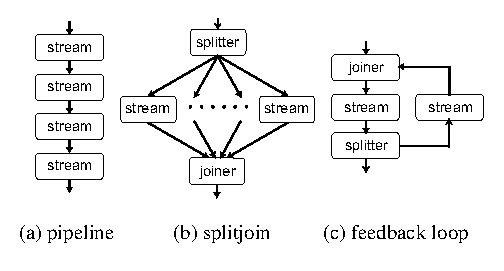
\includegraphics[scale=1, angle=0]{./constructs-eg.eps}
%}
% \vspace{-6pt}
% \nocaptionrule
 \caption{Hierarchical streams in StreamIt.}
 \label{fig:containers}
\end{center}
\end{figure}

\begin{figure}[t]
\begin{center}
\vspace{-12pt}
% \framebox{
 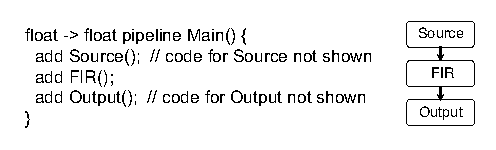
\includegraphics[scale=1, angle=0]{./pipeline-eg.eps}
%}
% \vspace{-6pt}
% \nocaptionrule
 \caption{Example pipeline with FIR filter.}
 \label{fig:pipeline}
%\vspace{-18pt}
\end{center}
\end{figure}

In StreamIt, the
application developer focuses on the hierarchical assembly of the
stream graph and its communication topology, rather than on the 
explicit management of the data buffers between filters.
StreamIt provides three hierarchical structures for composing filters
into larger stream graphs (see Figure~\ref{fig:containers}). The 
{\it pipeline} construct composes streams in sequence, with the output
of one connected to the input of the next.   An example of a pipeline
appears in Figure~\ref{fig:pipeline}.

The {\it splitjoin} construct distributes data to a set of parallel
streams, which are then joined together in a roundrobin fashion.  In
a splitjoin, the {\it splitter} performs the data scattering, and the
{\it joiner} performs the gathering. A splitter is a specialized
filter with a single input and  multiple output channels. On 
every execution step, it can distribute its output to any one of
its children in either a {\it duplicate} or a {\it roundrobin}
manner. For the former, incoming data are replicated to every
sibling connected to the splitter. For the latter, data are scattered
in a roundrobin manner, with each item sent to exactly one child
stream, in order.  The splitter type and the weights for distributing data to
child streams are declared as part of the syntax (e.g., \texttt{split
duplicate} or \texttt{split roundrobin($w_1,\ldots,w_n$)}). The
splitter counterpart is the joiner. It is a specialized filter with  
multiple input channels but only one output channel. The joiner
gathers data from its predecessors in a roundrobin manner (declared
as part of the syntax) to produce a single output stream.

StreamIt also provides a {\it feedback loop} construct for introducing
cycles in the graph.

%\section{Execution Model}
%\label{sec:execmodel}

%% A StreamIt program is represented by a hierarchical graph,
%% where the leaf nodes are filters, splitters, and joiners, and
%% the composite nodes are pipelines, splitjoins, and
%% feedback-loops. Edges in the graph represent data channels, which 
%% operate as FIFO queues.
\paragraph*{Execution Model}
As noted earlier, an actor (i.e., a filter, splitter, or joiner)
executes whenever there are enough data items on its input 
tape. In StreamIt, actors have  two epochs
of execution: one for initialization, and one for the {\it steady
state}. The initialization primes the input tapes to allow filters with
peeking to execute the very first instance of their work functions.
%%initialization in this setting is similar to the prologue stage in
%%software pipelining. 
A steady state is an execution that does not change the
buffering in the channels: the number of items on each channel
after the execution is the same as it was before the execution. 
Every valid stream graph has a steady state~\cite{LM87-i}, and within
a steady state, there are often many possibilities for interleaving
actor executions. 
%% The steady state schedule has the property that
%% the amount of data buffered between any two actors does not change
%% before and after the actor executions.
\begin{figure}[t]
\begin{center}
%%\vspace{-24pt}
%\vspace{24pt}
 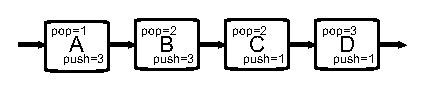
\includegraphics[scale=1, angle=0]{./pipe-with-rates.eps}
%\vspace{-6pt}
% \nocaptionrule
 \caption{Example pipeline.}
 \label{fig:pipe-with-rates}
\end{center}
%\vspace{-12pt}
\end{figure}
An example of a steady state for the pipeline in
Figure~\ref{fig:pipe-with-rates} requires filter \texttt{A} to fire
4 times, \texttt{B} 6 times, \texttt{C} 9 times, and
\texttt{D} 3 times. 
% Because in StreamIt the filters are
% independent (i.e., they do not share state), they can execute
% concurently. In a uniprocessor setting (which is what we use for our
% evaluation), we can only run one filter at time. Therefore, 
% The data generated by one actor are buffered (cached) until they are
% consumed.

\paragraph*{Compilation Process}
The StreamIt compiler derives the initialization and steady state
schedules~\cite{karczma-lctes03} and outputs a C program that includes
the initialization and work functions, as well as a driver to execute
each of the two schedules. Our compilation process allows the StreamIt
compiler to focus on high level optimizations, and relies on existing
compilers to perform machine-specific optimizations such as register
allocation, instruction scheduling, and 
code generation---this two-step approach affords us a
great deal of portability (e.g., code generated from the StreamIt
compiler is compiled and run on three different machines as reported
in Section~\ref{sec:evaluation}).

%% For example, referring to
%% Figure~\ref{fig:pipe-with-rates}, the compiler generates the following
%% sample code for running the steady state schedule:
%% %\begin{scriptsize}
%% \begin{verbatim}
%% run_steady_state() {
%%   for (i = 0; i < 4; i++) A_work();
%%   for (i = 0; i < 6; i++) B_work();
%%   for (i = 0; i < 9; i++) C_work();
%%   for (i = 0; i < 3; i++) D_work();
%% }
%% \end{verbatim}
%% %\end{scriptsize}
%% To execute the program, the steady state is wrapped with
%% another loop that invokes the steady state a designated number of
%% times. Preceding the state steady, a similar initialization schedule
%% is run to prime the data buffers.
%, and following the steady state, an
%epilogue is run to drain the buffers as necessary.

%% \begin{figure}[t]
%% \begin{center}
%% \vspace{-12pt}
%%  \psfig{figure=ssi.eps,width=3in}
%%  \vspace{-6pt}
%%  \caption{Instruction size (in bytes along the y-axis) per filter
%%  (x-axis) occurring in a steady state execution of FFT.}
%%  \label{fig:ssi-single}
%% \vspace{-18pt}
%% \end{center}
%% \end{figure}
